\section{Conclusions}
\subsection{Final Considerations}
The work carried out led to the development of an automatic summarization system capable of generating coherent summaries from food reviews. The system was designed to ensure ease of extension and adaptability to different types of tasks, thus increasing its versatility and potential applicability in varied contexts.\\
During the project, several automatic summarization models were implemented, including Seq2SeqLSTM, Seq2SeqBiLSTM, Seq2Seq3BiLSTM, and Seq2SeqGRU.
The results were evaluated through numerous metrics, such as ROUGE, Cosine Similarity, BERT score, and \texttt{MyEvaluation}. In particular,
BERT score proved to be the most representative metric of summary quality, as it considers the semantic context and similarity of words.\\

Furthermore, the \texttt{MyEvaluation} metric provided a more detailed assessment of summary quality, integrating various factors and assigning each a weight based on its relevance. Experimental results indicate that the \textbf{Seq2SeqBiLSTM} model achieved the best performance on almost all metrics,
suggesting a superior ability to capture semantic similarities between the generated summaries and the reference ones.
The \textbf{Seq2SeqBiLSTM} architecture achieved excellent results, obtaining on 1000 summaries:
\begin{table}[ht]
    \centering
    \rowcolors{2}{lightgray}{white}
    \begin{tabular}{@{} >{\bfseries}l c @{}}
        \toprule
        \textbf{Metric}    & \textbf{Value} \\
        \midrule
        ROUGE-1             & 0.16            \\
        ROUGE-2             & 0.03            \\
        ROUGE-L             & 0.16            \\
        Cosine similarity   & 41\%            \\
        BERT score           & 87\%            \\
        MyEvaluation        & 82\%            \\
        \bottomrule
    \end{tabular}
    \caption{Evaluation metrics}
\end{table}

It is important to underline that the results were influenced by the choice of dataset and the specific characteristics of the data,
including aspects related to preprocessing. These elements highlight the importance of careful selection and preparation of data to
optimize the performance of automatic summarization models.

\subsection{Testing the Best Model}
The \textbf{Seq2SeqBiLSTM} model showed superior performance compared to the other implemented models.\\
Below are some examples of summaries generated by the \textbf{Seq2SeqBiLSTM} model and their respective texts and reference summaries.\\

\begin{figure}[H]
    \centering
    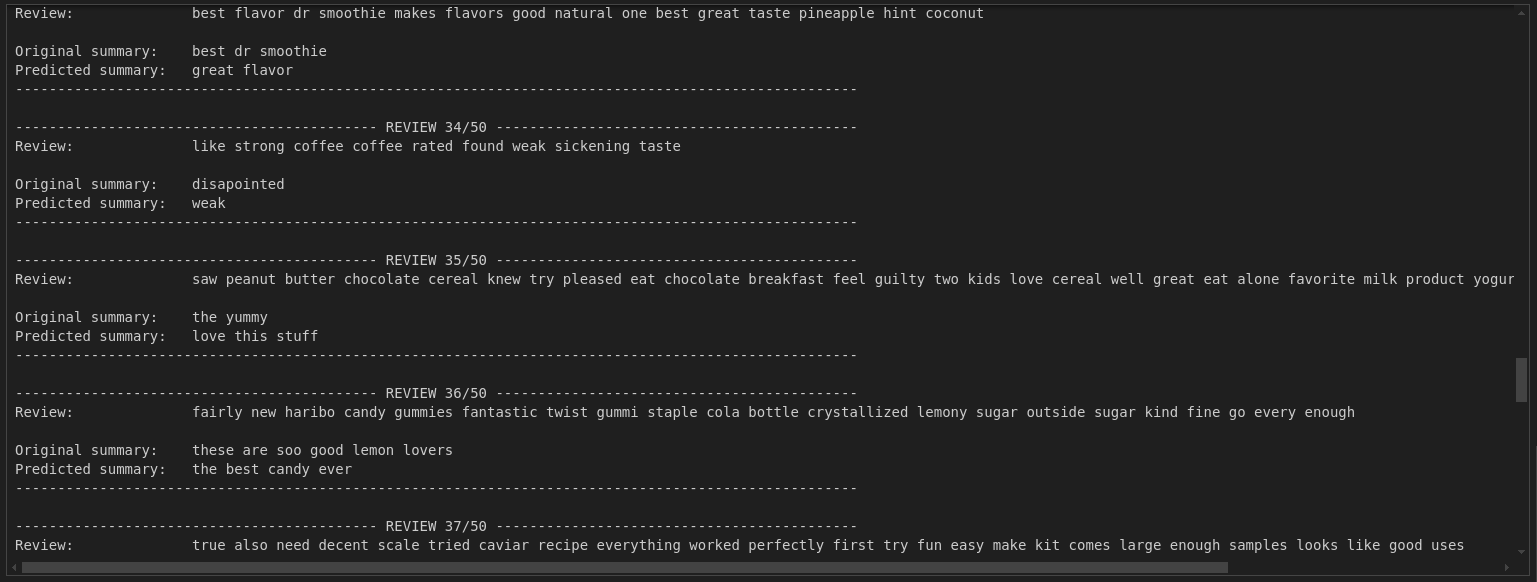
\includegraphics[width=0.75\textwidth]{media/Seq2SeqBiLSTM_inference.png}
    \caption{Example of summary generated by the Seq2SeqBiLSTM model}
    \label{fig:example1}
\end{figure}